\documentclass[a4paper,14pt]{extarticle}

\usepackage[utf8x]{inputenc}
\usepackage[T1,T2A]{fontenc}
\usepackage[russian]{babel}
\usepackage{hyperref}
\usepackage{indentfirst}
\usepackage{here}
\usepackage{array}
\usepackage{graphicx}
\usepackage{caption}
\usepackage{subcaption}
\usepackage{chngcntr}
\usepackage{amsmath}
\usepackage{amssymb}
\usepackage{pgfplots}
\usepackage{pgfplotstable}
\usepackage[left=2cm,right=2cm,top=2cm,bottom=2cm,bindingoffset=0cm]{geometry}
\usepackage{multicol}
\usepackage{askmaps}
\usepackage{titlesec}
\usepackage{listings}
\usepackage{color}
\usepackage{courier}

\definecolor{green}{rgb}{0,0.6,0}
\definecolor{gray}{rgb}{0.5,0.5,0.5}
\definecolor{purple}{rgb}{0.58,0,0.82}

\lstset{
	language=Verilog,
	backgroundcolor=\color{white},   
	basicstyle=\small\ttfamily,
	commentstyle=\color{green},
	keywordstyle=\color{blue},	
	numberstyle=\tiny\color{gray},
	stringstyle=\color{purple},
	breakatwhitespace=false,
	breaklines=true,
	captionpos=b,
	keepspaces=true,
	numbers=left,
	numbersep=5pt,
	showspaces=false,
	showstringspaces=false,
	showtabs=false,
	tabsize=4,
	frame=single,
	inputpath={../quartus/},
	literate={~} {$\sim$}{1}
}

\renewcommand{\le}{\ensuremath{\leqslant}}
\renewcommand{\leq}{\ensuremath{\leqslant}}
\renewcommand{\ge}{\ensuremath{\geqslant}}
\renewcommand{\geq}{\ensuremath{\geqslant}}
\renewcommand{\epsilon}{\ensuremath{\varepsilon}}
\renewcommand{\phi}{\ensuremath{\varphi}}
\renewcommand{\thefigure}{\arabic{figure}} 	
\renewcommand*\not[1]{\overline{#1}}

\titleformat*{\section}{\large\bfseries} 
\titleformat*{\subsection}{\normalsize\bfseries} 
\titleformat*{\subsubsection}{\normalsize\bfseries} 
\titleformat*{\paragraph}{\normalsize\bfseries} 
\titleformat*{\subparagraph}{\normalsize\bfseries} 

\counterwithin{figure}{section}
\counterwithin{equation}{section}
\counterwithin{table}{section}
\newcommand{\sign}[1][5cm]{\makebox[#1]{\hrulefill}}
\graphicspath{{../pics/}}
\captionsetup{justification=centering,margin=1cm}
\def\arraystretch{1.3}
\setlength\parindent{5ex}
\titlelabel{\thetitle.\quad}

\begin{document}

\begin{titlepage}
\begin{center}
	Санкт-Петербургский Политехнический Университет Петра Великого\\[0.3cm]
	Институт компьютерных наук и технологий \\[0.3cm]
	Кафедра компьютерных систем и программных технологий\\[4cm]
	
	\textbf{ОТЧЕТ}\\ 
	\textbf{по лабораторной работе}\\[0.5cm]
	\textbf{SystemVerilog №4}\\[0.1cm]
	Автоматизация проектирования\\ дискретных устройств\\[4.0cm]
\end{center}

\begin{flushright}
	\begin{minipage}{0.45\textwidth}
		\textbf{Работу выполнил студент}\\[3mm]
		группа 33501/4 \hspace*{9mm} Дьячков В.В.\\[5mm]
		\textbf{Преподаватель}\\[5mm]
		\sign[1.5cm] \hspace*{1mm} к.т.н., доц. Филиппов А.С. \\[5mm]
	\end{minipage}
\end{flushright}

\vfill

\begin{center}
	Санкт-Петербург\\
	\the\year
\end{center}
\end{titlepage}

\addtocounter{page}{1}
\counterwithin{lstlisting}{section}

\section*{Используемые сокращения}

\begin{itemize}
	\setlength{\itemsep}{0pt}
	\item FIFO -- First In First Out
	\item LVDS -- Low-Voltage Differencial Signaling
	\item PLL -- ФАПЧ (фазовая автоподстройка частоты)
	\item OSI/ISO -- Open Systems Interconnection (базовая эталонная модель взаимодействия открытых систем)
\end{itemize}

\newpage

\section*{Задание на курсовое проектирование}
\addcontentsline{toc}{section}{Задание на курсовое проектирование}

\subsection*{Краткое описание}
\addcontentsline{toc}{subsection}{Краткое описание}

Устройство передачи данных решает три укрупненных задачи:
\begin{enumerate}
	\item Прием и буферизация данных от нескольких источников синхронных сигналов (синхросигнал расположен фронтом по центру бита, фазовый разброс $\pm1$ нс). Поток входных данных идет непрерывно.
	\item Когда в буфере FIFO накапливаются данные, достаточные для формирования пакета, устройство управления выдает команду блоку коммутации и формирования пакета, который формирует пакет в соответствии с заданием. Если данные для передачи отсутствуют, передается "пустой" пакет с отсутствующими данными, \code{M = 0} по каналу \code{N = 15}.
	\item LVDS Transmitter -- передатчик LVDS канала обеспечивает передачу синхронных дифференциальных данных по заданному числу каналов (Number of Channels) с заданной скоростью передачи (Output data rate).
\end{enumerate}

Укрупненная структурная схема устройства передачи данных.
\begin{figure}[H]
	\centering
	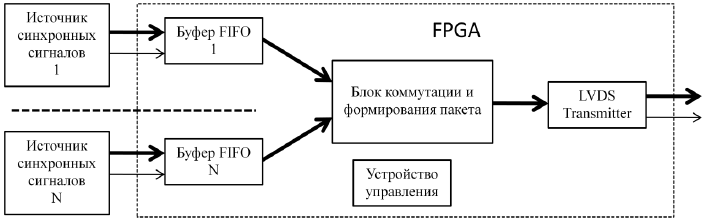
\includegraphics[width=\linewidth]{structure}
\end{figure}

\subsection*{Решаемые задачи}
\addcontentsline{toc}{subsection}{Решаемые задачи}

\begin{itemize}

	\item Анализ технического задания
	\begin{itemize}
		\item Анализ вариантов реализации и разработка структурной семы устройства.
		\item Детализация структурных блоков, разработка функциональной схемы устройства.
		\item Анализ IP-функций, используемых в устройстве, формирование требований к разрабатываемым блокам.
			\begin{itemize}
				\item[$\circ$] \code{FIFO}
				\item[$\circ$] \code{ALTLVDS_TX}\\[5mm]
			\end{itemize}
	\end{itemize}
	
	\item Разработка функционально-логического описания и моделирование
	\begin{itemize}
		\item Организация FIFO.
		\item Организация и настройка передатчика LVDS.
		\item Разработка блока коммутации.
		\item Разработка устройства управления.
		\item Интеграция разработанных блоков и моделирование работы устройства передачи данных.
	\end{itemize}
	
	
	\item Верификация устройства передачи данных в системном окружении
	\begin{itemize}
		\item Разработка имитатора системного окружения, задающего поток входных данных.
		\item Создание и настройка средств системной отладки.
		\item Исследование работы устройства передачи данных на плате-прототипе (Mini DiLab).
	\end{itemize}

\end{itemize}

\subsection*{Вариант индивидуального задания}
\addcontentsline{toc}{subsection}{Вариант индивидуального задания}

\begin{itemize}
	\item Три 16-разрядных источника сигналов, частота 10 МГц;
	\item Количество байт данных \code{M = 9};
	\item Формат пакета: <<\code{H1MD}>> (\code{H1} -- первый байт заголовка \code{0xFN}, где \code{N} -- номер канала; \code{M} -- количество байт данных; \code{D} -- передаваемые данные);
 	\item Двухканальный LVDS передатчик, скорость передачи данных $600$ Мб/с.
\end{itemize}

\newpage

\section*{Введение}
\addcontentsline{toc}{section}{Введение}

Передача данных -- физический перенос данных (цифрового битового потока) в виде сигналов от точки к точке или от точки к нескольким точкам средствами электросвязи по каналу передачи данных. Обычно принятые данные обрабатываются средствами вычислительной техники. Примерами каналов передачи могут служить медные провода, волоконно-оптическая линия передачи, беспроводные каналы передачи данных или запоминающее устройство.

Передаваемые данные могут быть цифровыми сообщениями, идущими из источника данных, например, из компьютера или от клавиатуры. Это может быть и аналоговый сигнал — телефонный звонок или видеосигнал, оцифрованный в битовый поток, используя импульсно-кодирующую модуляцию (PCM) или более расширенные схемы кодирования источника (аналого-цифровое преобразование и сжатие данных). Кодирование источника и декодирование осуществляется кодеком или кодирующим оборудованием.

В проекте рассмотрено устройство передачи данных, принимающее данные с нескольких источников синхронных сигналов с непрерывным потоком. Разработанное устройство должно формировать пакеты для отправки их далее в канал связи с использование LVDS передатчика.

\newpage

\tableofcontents

\newpage

\section{Разработка устройства передачи данных}

\subsection{Общая схема устройства}

\subsection{Входной буфер}

\subsection{Блок коммутации и формирования пакета}

\subsection{LVDS передатчик}

\subsection{Компиляция проекта. Проверка временных требований}

\newpage

\section{Моделирование работы устройства}

\subsection{Буфер входных данных}

На рис. \ref{fig:input_buffer_modelling} приведены результаты моделирования буфера входных данных.
\begin{figure}[H]
	\centering
	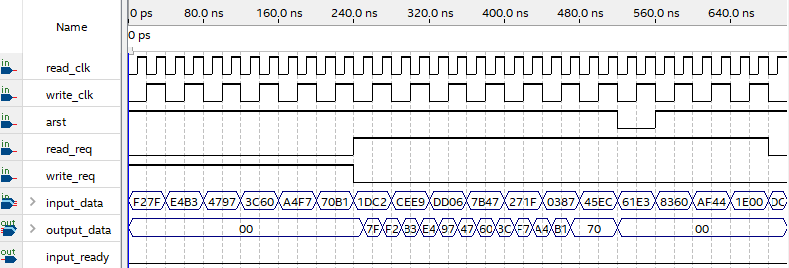
\includegraphics[width=\linewidth]{input_buffer/modelling}
	\caption{Результаты моделирования буфера входных данных}
	\label{fig:input_buffer_modelling}
\end{figure}

\subsection{Блок коммутации и формирования пакета}

На рис. \ref{fig:commutator_modelling} приведены результаты моделирования блока коммутации.
\begin{figure}[H]
	\centering
	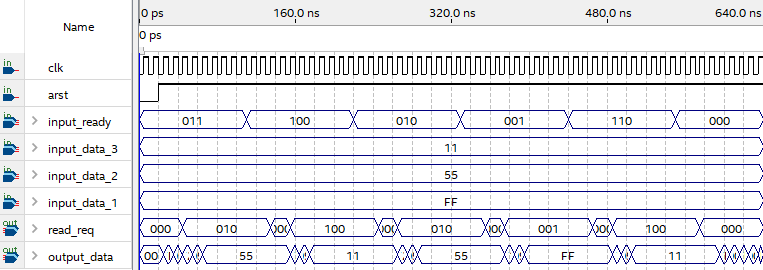
\includegraphics[width=\linewidth]{commutator/modelling}
	\caption{Результаты моделирования блока коммутации}
	\label{fig:commutator_modelling}
\end{figure}

\subsubsection{Дешифратор номера канала}

На рис. \ref{fig:channel_encoder_modelling} приведены результаты моделирования дешифратора номера канала.
\begin{figure}[H]
	\centering
	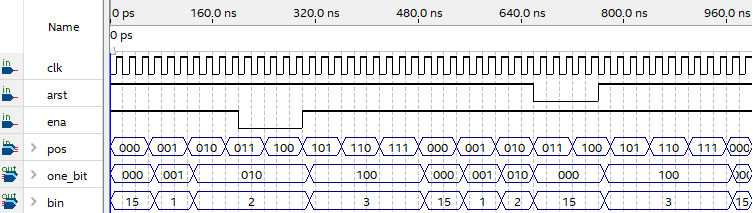
\includegraphics[width=\linewidth]{channel_encoder/modelling}
	\caption{Результаты моделирования дешифратора номера канала}
	\label{fig:channel_encoder_modelling}
\end{figure}

\subsubsection{Мультиплексор входных данных}

На рис. \ref{fig:input_muxer_modelling} приведены результаты моделирования мультиплексора входных данных.
\begin{figure}[H]
	\centering
	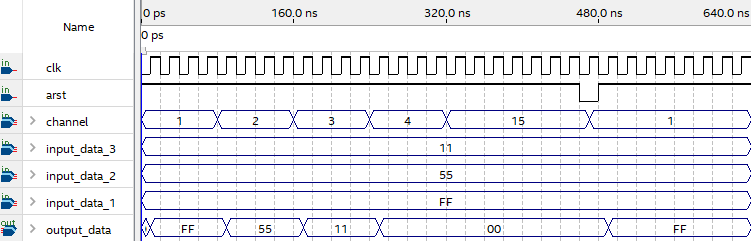
\includegraphics[width=\linewidth]{input_muxer/modelling}
	\caption{Результаты моделирования мультиплексора входных данных}
	\label{fig:input_muxer_modelling}
\end{figure}

\subsubsection{Устройство управления}

На рис. \ref{fig:control_unit_modelling} приведены результаты моделирования устройства управления.
\begin{figure}[H]
	\centering
	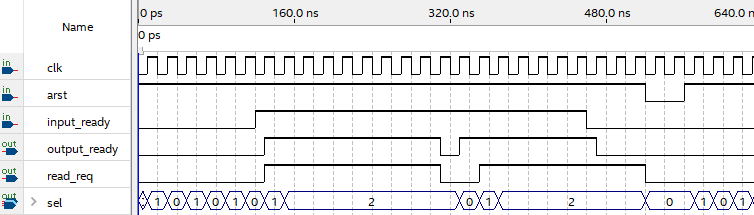
\includegraphics[width=\linewidth]{control_unit/modelling}
	\caption{Результаты моделирования устройства управления}
	\label{fig:control_unit_modelling}
\end{figure}

\subsubsection{Мультиплексор выходных данных}

На рис. \ref{fig:output_muxer_modelling} приведены результаты моделирования мультиплексора выходных данных.
\begin{figure}[H]
	\centering
	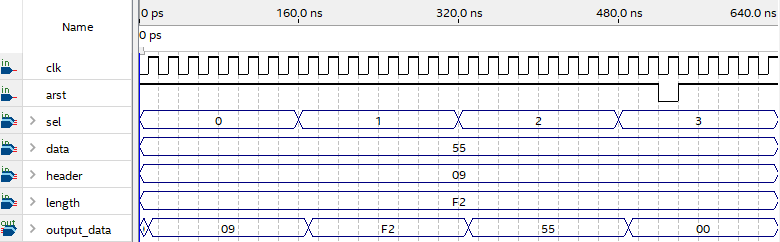
\includegraphics[width=\linewidth]{output_muxer/modelling}
	\caption{Результаты моделирования мультиплексора выходных данных}
	\label{fig:output_muxer_modelling}
\end{figure}

\subsection{LVDS передатчик}

На рис. \ref{fig:lvds_transmitter_modelling} приведены результаты моделирования LVDS передатчика.
\begin{figure}[H]
	\centering
	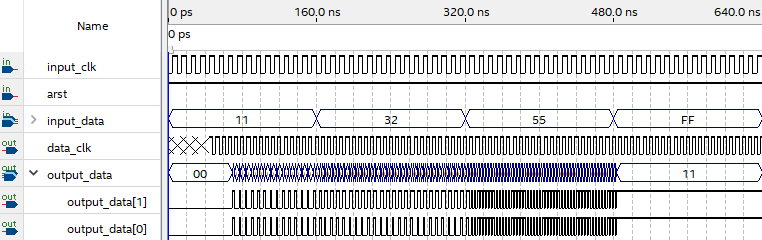
\includegraphics[width=\linewidth]{lvds_transmitter/modelling}
	\caption{Результаты моделирования LVDS передатчика}
	\label{fig:lvds_transmitter_modelling}
\end{figure}

\subsection{Устройство передачи данных}

На рис. \ref{fig:transmitter_modelling} приведены результаты моделирования устройства передачи данных.
\begin{figure}[H]
	\centering
	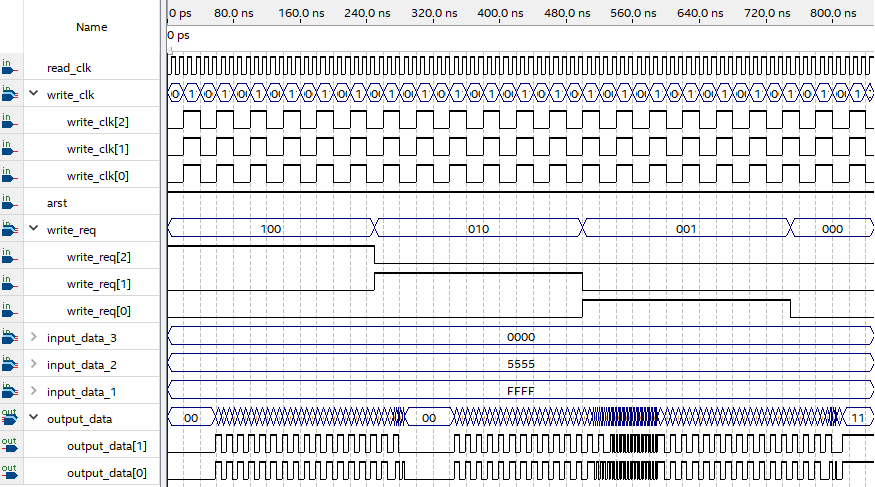
\includegraphics[width=\linewidth]{transmitter/modelling}
	\caption{Результаты моделирования устройства передачи данных}
	\label{fig:transmitter_modelling}
\end{figure}

\newpage

\section*{Заключение}
\addcontentsline{toc}{section}{Заключение}

\newpage

\section*{Список используемой литературы}
\addcontentsline{toc}{section}{Список используемой литературы}

\begin{enumerate}
	\item FIFO Intel ®FPGA IP User Guide // [Электронный ресурс.] --\\
	URL: \href{https://www.altera.com/en_US/pdfs/literature/ug/ug_fifo.pdf}{https://www.altera.com/en\_US/pdfs/literature/ug/ug\_fifo.pdf}\\
	(дата обращения: 01.06.2018)
	\item LVDS SERDES Transmitter / Receiver IP Cores User Guide // [Электронный ресурс.] --\\
	URL: \href{https://www.altera.com/en_US/pdfs/literature/ug/ug_altlvds.pdf}{https://www.altera.com/en\_US/pdfs/literature/ug/ug\_altlvds.pdf}\\
	(дата обращения: 02.06.2018)
	\item Altera Phase-Locked Loop (Altera PLL) IP Core User Guide // [Электронный ресурс.] --\\
	URL: \href{https://www.altera.com/en_US/pdfs/literature/ug/altera_pll.pdf}{https://www.altera.com/en\_US/pdfs/literature/ug/altera\_pll.pdf}\\
	(дата обращения: 03.06.2018)
\end{enumerate}

\newpage

\section*{Приложение 1. Исходный код на языке Verilog}
\addcontentsline{toc}{section}{Приложение 1. Исходный код на языке Verilog}

\subsection*{Буфер входных данных}

\lstinputlisting[caption=\code{input_buffer.v}]{input_buffer.v}

\subsection*{Блок коммутации и формирования пакета}

\lstinputlisting[caption=\code{commutator.v}]{commutator.v}

\newpage

\subsection*{Шифратор номера канала}

\lstinputlisting[caption=\code{channel_encoder.v}]{channel_encoder.v}

\subsection*{Мультиплексор входных данных}

\lstinputlisting[caption=\code{input_muxer.v}]{input_muxer.v}

\subsection*{Устройство управления}

\lstinputlisting[caption=\code{control_unit.v}]{control_unit.v}

\subsection*{Мультиплексор выходных данных}

\lstinputlisting[caption=\code{output_muxer.v}]{output_muxer.v}

\newpage

\subsection*{LVDS передатчик}

\lstinputlisting[caption=\code{output_buffer.v}]{lvds_transmitter.v}

\subsection*{Устройство передачи данных}

\lstinputlisting[caption=\code{transmitter.v}]{transmitter.v}

\end{document}